%!TEX root = ../dokumentation.tex

\chapter{Theoretische Grundlagen}
\section{Frequenzbereiche in der Funktechnik}
\begin{figure}[ht]
	\centering
	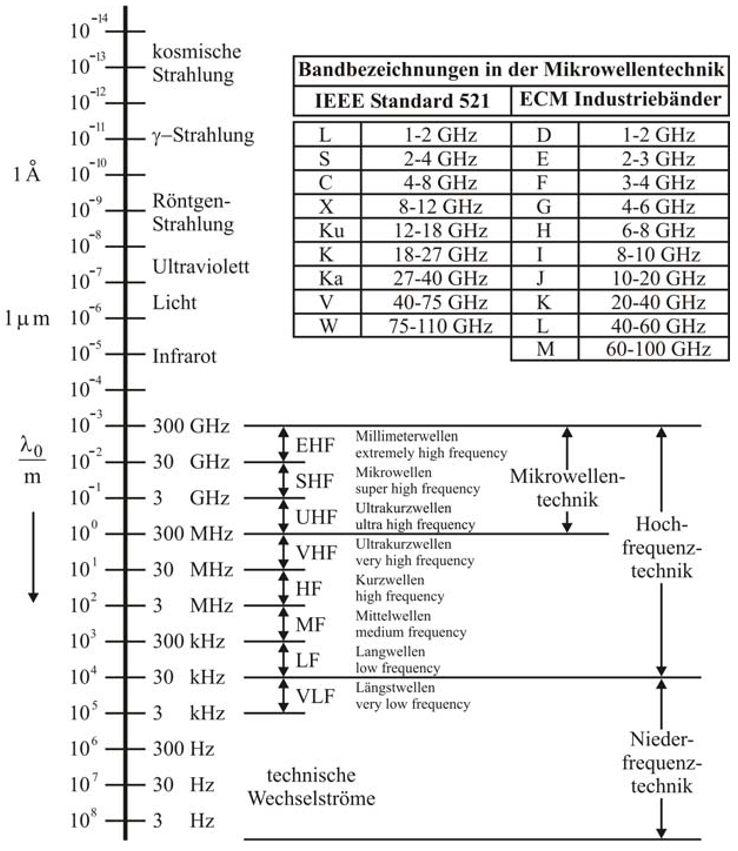
\includegraphics[width=0.75\textwidth]{frequenzbereich.png}
	\caption[Spektrum elektromagnetischer Wellen und gebräuchliche Bandbezeichnungen]{Spektrum elektromagnetischer Wellen und gebräuchliche Bandbezeichnungen. Quelle: \cite[Kark, S. 1]{Kark2006}} 
	\label{frequenzbereiche}
\end{figure}



Die Aufteilung des Frequenzbereiches von 0 kHz bis 3000 GHz wird von der Bundesnetzagentur im sogenannten Frequenzplan \cite[Bundesnetzagentur, 2016]{bundesnetzagentur-frequenzplan:2016} gemäß § 54 TKG festgehalten.

\section{Bluetooth}
Bluetooth ist eine Übertragungstechnik für kabellose Kommunikation über kurze Distanzen. Es wird im Frequenzbereich von 2,4 bis 2,4835 GHz betrieben \cite[Bundesamt für Strahlenschutz, S. 1]{bundesamt-strahlungsschutz:2012}. Insgesamt gibt es unter Bluetoothgeräten drei verschiedene Sendeleistungsklassen:
\begin{description}
	\item[Klasse 1: bis 1,0 mW] Reichweite: bis 10m 
	\item [Klasse 2: bis 2,5 mW] Reichweite: 10m und mehr
	\item [Klasse 3: bis 100 mW] Reichweite: 100m und mehr
\end{description}
Die Aufteilung des Frequenzbereiches von 0 kHz bis 3000 GHz wird von der Bundesnetzagentur im sogenannten Frequenzplan \cite[Bundesnetzagentur]{bundesnetzagentur-frequenzplan:2016} gemäß § 54 TKG festgehalten.
\section{Dezimeterwelle}


